\section{GT2 and GT5: The Kovacs Witness and What It Costs to Repair}
\label{sec:gt2-gt5}
%% Packet W-04. Ledger rows: GT2, GT5, NEG.gt2_loop_certificate_not_built.

\subsection{The Kovacs protocol on the audited class}

The Kovacs protocol \cite{kovacs-1963} (equilibrate hot, quench cold, age for $t_w$, jump up to
an intermediate temperature, watch a one-time observable relax) was located on the East substrate
by an exact search, run before any certificate and filed as a pre-certificate control. At $N=10$,
$\epsilon: 7/10 \to 1/10 \to 2/5$ with $t_w = 40$, the mean energy after the second jump starts
below its new equilibrium value $20/7 \approx 2.857$ (at $\approx 2.741$), crosses it between
steps $1$ and $2$ ($\approx 2.803$ and $\approx 2.859$), and overshoots through a hump peaking at
$t_{\mathrm{peak}} = 35$ before returning (Fig.~\ref{fig:kovacs-hump}), all in exact rational
arithmetic; $t_K = 1$ denotes the last step before the crossing. The raw trace never equals
$20/7$ at an integer step; the preparation that does, a randomized stop between steps $1$ and $2$,
is constructed in \S\ref{sec:gt2-witness}. The non-monotone excursion after the crossing is the
classic signature that the present value does not determine the future; for a finite Markov chain
in the linear-response regime, Prados and Brey showed it is generic whenever the observable's
relaxation is not a single exponential \cite{prados-brey-2010}. That East- and FA-type models show a Kovacs hump was established
numerically by \cite{buhot-2003,arenzon-sellitto-2004}; what is new here is the exact-rational
trace and the certificate built on it.

\begin{figure}[htbp]
  \centering
  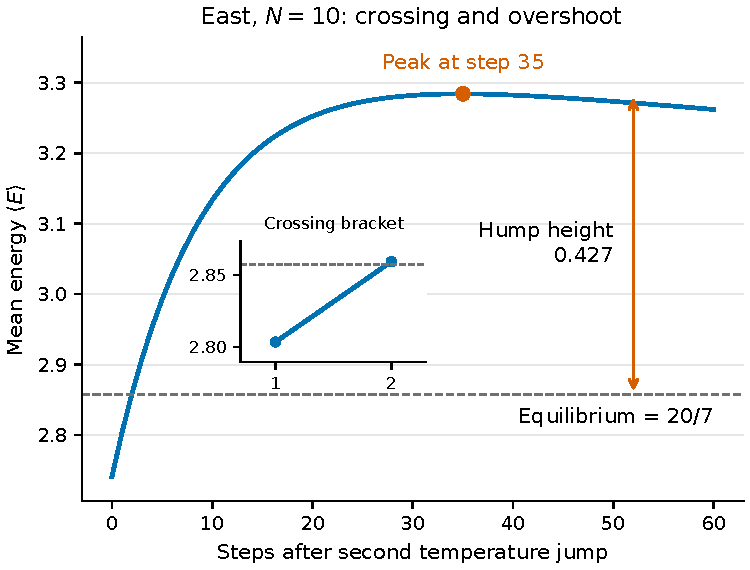
\includegraphics[width=0.7\linewidth]{figures/out/fig_gt2_kovacs_hump.pdf}
  \caption{Kovacs hump on East $N=10$ (exact-rational trace, floats only for plotting): the mean
    energy starts below its equilibrium value $20/7$, crosses it between steps $1$ and $2$
    (inset), peaks at step $35$, and returns toward equilibrium.}
  \label{fig:kovacs-hump}
\end{figure}

\subsection{GT2: the witness certificate}
\label{sec:gt2-witness}

In plain terms: we exhibit two preparation histories of the East chain with exactly the same
present mean energy and provably different mean energies five steps later. The first history is
the Kovacs run stopped at the crossing: since no single time step lands exactly on $20/7$, the
run is stopped at step $1$ with probability $\theta \approx 0.0359$ and at step $2$ otherwise,
with $\theta$ solved exactly so that the mixture's mean energy is $20/7$ (a ``randomized stop'',
a declared move of the pipeline). The second history is the equilibrium distribution at
$\epsilon = 2/5$, whose mean energy is $20/7$ by definition. Both are then held at
$\epsilon = 2/5$ for five steps and their mean energies compared: the equilibrium history stays
at $20/7 \approx 2.857$ while the Kovacs history has moved to $\approx 3.058$, a gap of
$\approx 0.201$. Only the mean energy is matched at the start, not the full energy distribution;
that is exactly what the energy readout, as a lens, sees. Precisely:

\claimref{GT2}{321f9bffdbf1368ec764a8fcde97d569dd9f4292ee5a98a0b6f30ac9483ce7bf}
On the declared scope (East, $N=10$, \texttt{kovacs\_moment} lens, declared $\epsilon$ grid and
continuation catalog), one exact-rational split pair of preparation histories is exhibited: the
two histories agree on the present lens value (mean energy $20/7$) and their futures differ, with
an exact maximum absolute future gap that is a strictly positive rational number
($\approx 0.2005$ on the five-step hold; the exact fraction is in the artifact). By
\sbtcite{sbt-paper-a} Thm.~3.5, the existence of such a pair is equivalent to the comparison map
$\pi: M \to Q$ being strictly refining, that is, to the predictive description being genuinely
finer than the present-observable one. Grade: theorem (audited class).

The framework distinguishes three things a ``different future'' could mean, and we claim only the
first: that the future depends on more than the present readout; \emph{not} that the two
histories took different routes to the same state (a P3 route mismatch); and \emph{not} any
directionality or irreversibility. In the framework's filing vocabulary the first reading is
\textbf{P4 staged-dependence}, filed on the standard witness template (F-II
\texttt{prop:p1-witness}). No P6\_drive audit was performed, so no arrow-of-time statement of any kind is
made on GT2's behalf.

\claimref{NEG.gt2\_loop\_certificate\_not\_built}{321f9bffdbf1368ec764a8fcde97d569dd9f4292ee5a98a0b6f30ac9483ce7bf}
The proposal also called for a companion certificate about thermal loops (a closed temperature
cycle acting trivially on the present description $Q$ but nontrivially on the predictive
description $M$). It was not built: the split-pair witness stands alone, and, as
\S\ref{sec:lean} makes precise, the vendored formal core cannot even express a non-vacuous
loop-asymmetry instance, so a computational loop certificate would first need new formal footing.
Disclosed here and in the gap register; nothing downstream depends on it.

\subsection{GT5: what it costs to buy the distinction back}

In plain terms: adding a single scalar to the energy readout is enough to tell the two witness
histories apart, and a fictive-temperature-like index is one of three declared choices that
work. Precisely:

\claimref{GT5}{746b44e6c2f7f92364137a202f7306b6afc9e99c413fb4dd3a40d47bfd6f94c8}
On the declared scope (East, $N=10$, \texttt{kovacs\_moment} interface, the declared two-history
class), the present lens collapses the witness pair into one class ($|Q| = 1$ on the pair) while
the predictive quotient keeps two ($|M| = 2$), so the largest fiber of $\pi$ has size
$\mathrm{MaxFiber} = 2$, meeting the nontriviality threshold. The buyback curve
(Fig.~\ref{fig:buyback}) is published as a lift ledger per F-II \texttt{prop:forgetting-lifts}:
each added memory coordinate is a recorded, selected, non-unique lift. At budget $0$ the pair is
unresolved; at budget $1$, \emph{each} of the three declared scalar coordinates already resolves
it exactly (loss $0/1$), so the shipped witness saturates at $\texttt{saturation\_budget} = 1$.
The three coordinates are expectations over the history's microstate distribution $\mu$ of a
per-microstate quantity: $T_f(\mu) = \mathbb{E}_\mu[\,i^*(E(n))\,]$, where $i^*(E)$ is the
index of the grid value $\epsilon_i$ whose equilibrium mean energy is closest to $E$ (an index
into the declared grid, not a temperature, and not inferred from the history's mean energy, so
two histories with equal mean energy can have different $T_f$); $D(\mu)$, the expected number
of adjacent up-up spin pairs; and $n_1(\mu)$, the expected occupation of the site next to the
wall.

The translation to the glass literature is deliberately modest. The TNM fictive temperature
\cite{tool-1946,narayanaswamy-1971,moynihan-1976,hodge-1994} is the motivating analogy for $T_f$: an
energy-indexed effective temperature added as a declared step from the present description
toward the predictive one. The implemented $T_f$ is the grid-index construction above, not the
TNM quantity itself. Modern treatments of the Kovacs effect likewise pair an effective
temperature with a second structural variable \cite{bouchbinder-langer-2010}, and the
multiparameter models the Kovacs literature moved to \cite{kahr-1979} are why the general
insufficiency question is left open here rather than answered on one pair. For
\emph{this} minimal two-history witness, one scalar suffices; the certificate demonstrates the
repair \emph{mechanism} and its ledger discipline. It is not a claim that a single
fictive-temperature-like scalar is insufficient in general: such a claim would require a richer
multi-instance construction that was not built here.

\begin{figure}[htbp]
  \centering
  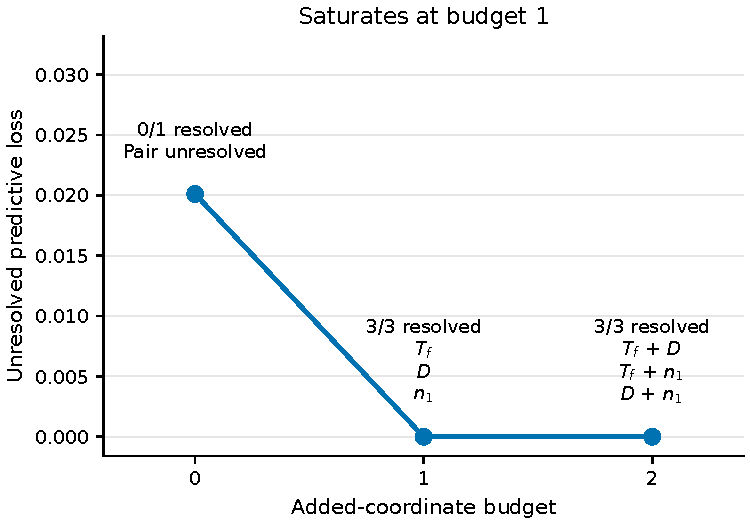
\includegraphics[width=0.7\linewidth]{figures/out/fig_gt5_buyback.pdf}
  \caption{GT5 buyback curve: unresolved predictive loss versus added-coordinate budget, annotated
    with resolved/attempted counts and the resolving coordinates. The loss is the budget envelope
    of the two-point squared prediction error $(a-b)^2/2$, where $a$ and $b$ are the two
    histories' five-step future mean energies, incurred only while the pair is left in one class
    ($\approx 0.0201$ at budget $0$, i.e.\ half the squared witness gap); a group that separates
    the pair has loss $0$. The shipped two-history witness saturates at budget $1$.}
  \label{fig:buyback}
\end{figure}
